\documentclass[a4paper,12pt]{article} 

% First, we usually want to set the margins of our document. For this we use the package geometry.
\usepackage[top = 2.5cm, bottom = 2.5cm, left = 2.5cm, right = 2.5cm]{geometry} 
\usepackage[T1]{fontenc}
\usepackage[utf8]{inputenc}

% The following two packages - multirow and booktabs - are needed to create nice looking tables.
\usepackage{multirow} % Multirow is for tables with multiple rows within one cell.
\usepackage{booktabs} % For even nicer tables.

% As we usually want to include some plots (.pdf files) we need a package for that.
\usepackage{graphicx} 

% The default setting of LaTeX is to indent new paragraphs. This is useful for articles. But not really nice for homework problem sets. The following command sets the indent to 0.
% \usepackage{setspace}
% \setlength{\parindent}{0in}
\usepackage{indentfirst}


% Package to place figures where you want them.
\usepackage{float}

% The fancyhdr package let's us create nice headers.
\usepackage{fancyhdr}

\usepackage{amsmath,amsthm,tikz}
\usetikzlibrary{automata,positioning}

% To make our document nice we want a header and number the pages in the footer.

\pagestyle{fancy} % With this command we can customize the header style.

\fancyhf{} % This makes sure we do not have other information in our header or footer.

\lhead{\footnotesize Data Structure and Algorithm Analysis(H): Work Sheet 15}% \lhead puts text in the top left corner. \footnotesize sets our font to a smaller size.

%\rhead works just like \lhead (you can also use \chead)
\rhead{\footnotesize Mengxuan Wu} %<---- Fill in your lastnames.

% Similar commands work for the footer (\lfoot, \cfoot and \rfoot).
% We want to put our page number in the center.
\cfoot{\footnotesize \thepage} 

\begin{document}

\thispagestyle{empty} % This command disables the header on the first page. 

\begin{tabular}{p{15.5cm}}
{\large \bf Data Structure and Algorithm Analysis(H)} \\
Southern University of Science and Technology \\ Mengxuan Wu \\ 12212006 \\
\hline
\\
\end{tabular}

\vspace*{0.3cm} %add some vertical space in between the line and our title.

\begin{center}
	{\Large \bf Work Sheet 15}
	\vspace{2mm}

	{\bf Mengxuan Wu}
		
\end{center}  

\vspace{0.4cm}

\section*{Question 15.1}

\subsection*{Prim's Algorithm}

Suppose we begin with the vertex $a$.
\begin{center}
	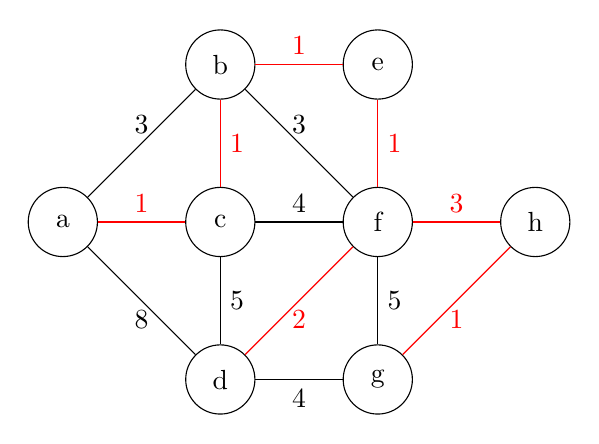
\begin{tikzpicture}[auto]
		\draw (0,0) node [state] (a) {a};
		\draw (2,2) node [state] (b) {b};
		\draw (2,0) node [state] (c) {c};
		\draw (2,-2) node [state] (d) {d};
		\draw (4,2) node [state] (e) {e};
		\draw (4,0) node [state] (f) {f};
		\draw (4,-2) node [state] (g) {g};
		\draw (6,0) node [state] (h) {h};

		\draw 
		    (a) edge [color=red] node [above] {1} (c)
			(c) edge [color=red] node [right] {1} (b)
			(b) edge [color=red] node [above] {1} (e)
			(e) edge [color=red] node [right] {1} (f)
			(f) edge [color=red] node [below] {2} (d)
			(f) edge [color=red] node [above] {3} (h)
			(h) edge [color=red] node [below] {1} (g)
			(a) edge node [above] {3} (b)
			(a) edge node [below] {8} (d)
			(b) edge node [above] {3} (f)
			(c) edge node [above] {4} (f)
			(c) edge node [right] {5} (d)
			(d) edge node [below] {4} (g)
			(f) edge node [right] {5} (g)
		;
	\end{tikzpicture}
\end{center}

Edges with order considered:
\begin{center}
	\begin{tabular}{ccc}
		\toprule
		Edge & Weight & Order \\
		\midrule
		$ac$ & 1 & 1 \\
		$cb$ & 1 & 2 \\
		$be$ & 1 & 3 \\
		$ef$ & 1 & 4 \\
		$fd$ & 2 & 5 \\
		$fh$ & 3 & 6 \\
		$hg$ & 1 & 7 \\
		\bottomrule
	\end{tabular}
\end{center}

The total weight is 10.

\subsection*{Kruskal's Algorithm}

\begin{center}
	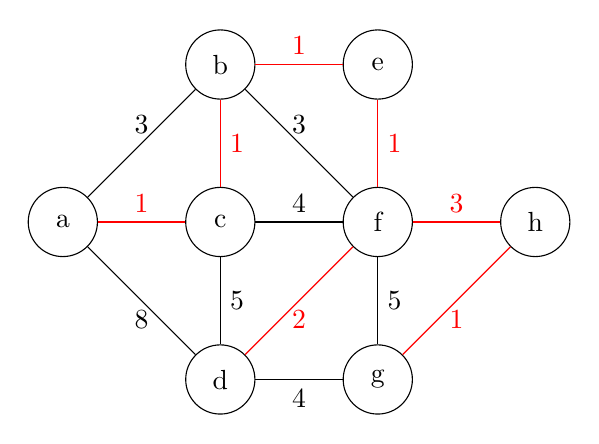
\begin{tikzpicture}[auto]
		\draw (0,0) node [state] (a) {a};
		\draw (2,2) node [state] (b) {b};
		\draw (2,0) node [state] (c) {c};
		\draw (2,-2) node [state] (d) {d};
		\draw (4,2) node [state] (e) {e};
		\draw (4,0) node [state] (f) {f};
		\draw (4,-2) node [state] (g) {g};
		\draw (6,0) node [state] (h) {h};

		\draw 
		    (a) edge [color=red] node [above] {1} (c)
			(c) edge [color=red] node [right] {1} (b)
			(b) edge [color=red] node [above] {1} (e)
			(e) edge [color=red] node [right] {1} (f)
			(f) edge [color=red] node [below] {2} (d)
			(f) edge [color=red] node [above] {3} (h)
			(h) edge [color=red] node [below] {1} (g)
			(a) edge node [above] {3} (b)
			(a) edge node [below] {8} (d)
			(b) edge node [above] {3} (f)
			(c) edge node [above] {4} (f)
			(c) edge node [right] {5} (d)
			(d) edge node [below] {4} (g)
			(f) edge node [right] {5} (g)
		;
	\end{tikzpicture}
\end{center}

Edges with order considered:
\begin{center}
	\begin{tabular}{ccc}
		\toprule
		Edge & Weight & Order \\
		\midrule
		$ac$ & 1 & 1 \\
		$cb$ & 1 & 2 \\
		$be$ & 1 & 3 \\
		$ef$ & 1 & 4 \\
		$hg$ & 1 & 5 \\
		$fd$ & 2 & 6 \\
		$fh$ & 3 & 7 \\
		\bottomrule
	\end{tabular}
\end{center}

The total weight is 10.

\section*{Question 15.2}

\textbf{Step 1:}
\begin{center}
	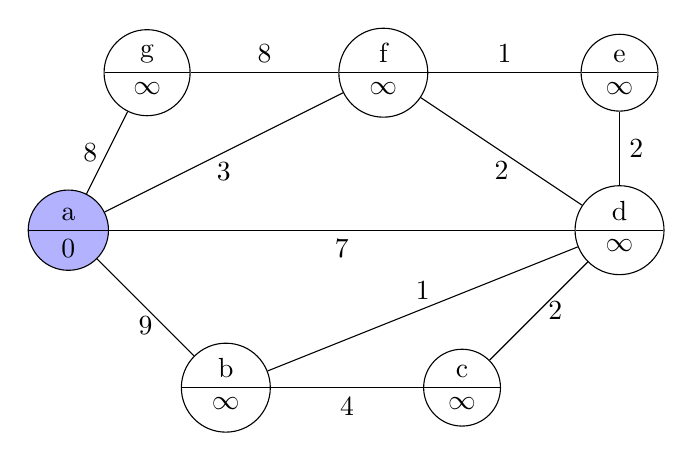
\begin{tikzpicture}
		\draw (0,0) node [state with output, fill=blue!30] (a) {a \nodepart{lower} 0};
		\draw (2,-2) node [state with output] (b) {b \nodepart{lower} $\infty$};
		\draw (5,-2) node [state with output] (c) {c \nodepart{lower} $\infty$};
		\draw (7,0) node [state with output] (d) {d \nodepart{lower} $\infty$};
		\draw (7,2) node [state with output] (e) {e \nodepart{lower} $\infty$};
		\draw (4,2) node [state with output] (f) {f \nodepart{lower} $\infty$};
		\draw (1,2) node [state with output] (g) {g \nodepart{lower} $\infty$};

		\draw
			(a) edge node [below] {9} (b)
			(a) edge node [left] {8} (g)
			(a) edge node [below] {3} (f)
			(b) edge node [below] {4} (c)
			(c) edge node [right] {2} (d)
			(d) edge node [right] {2} (e)
			(d) edge node [below] {2} (f)
			(e) edge node [above] {1} (f)
			(f) edge node [above] {8} (g)
			(a) edge node [below] {7} (d)
			(b) edge node [above] {1} (d)
		;
	\end{tikzpicture}
\end{center}

\newpage
\textbf{Step 2:}
\begin{center}
	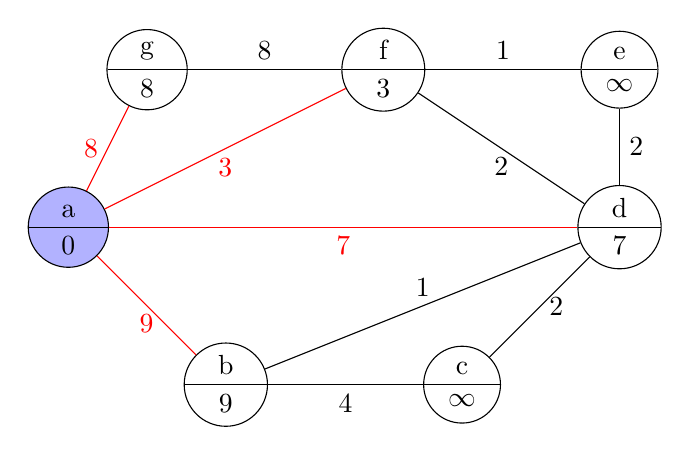
\begin{tikzpicture}
		\draw (0,0) node [state with output, fill=blue!30] (a) {a \nodepart{lower} 0};
		\draw (2,-2) node [state with output] (b) {b \nodepart{lower} 9};
		\draw (5,-2) node [state with output] (c) {c \nodepart{lower} $\infty$};
		\draw (7,0) node [state with output] (d) {d \nodepart{lower} 7};
		\draw (7,2) node [state with output] (e) {e \nodepart{lower} $\infty$};
		\draw (4,2) node [state with output] (f) {f \nodepart{lower} 3};
		\draw (1,2) node [state with output] (g) {g \nodepart{lower} 8};

		\draw
			(a) edge [color=red] node [below] {9} (b)
			(a) edge [color=red] node [left] {8} (g)
			(a) edge [color=red] node [below] {3} (f)
			(b) edge node [below] {4} (c)
			(c) edge node [right] {2} (d)
			(d) edge node [right] {2} (e)
			(d) edge node [below] {2} (f)
			(e) edge node [above] {1} (f)
			(f) edge node [above] {8} (g)
			(a) edge [color=red] node [below] {7} (d)
			(b) edge node [above] {1} (d)
		;
	\end{tikzpicture}
\end{center}

\textbf{Step 3:}
\begin{center}
	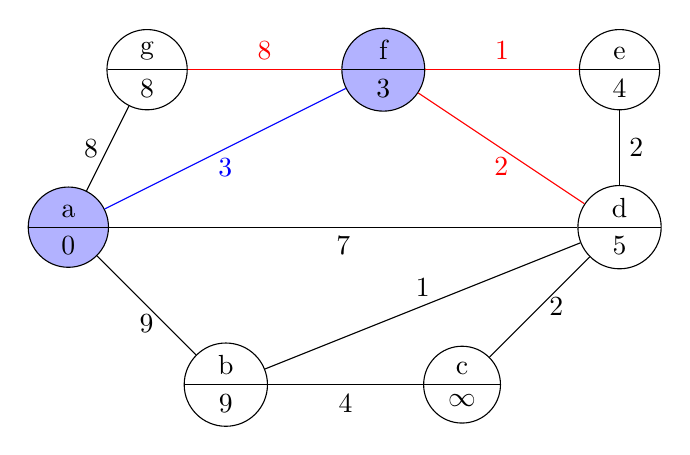
\begin{tikzpicture}
		\draw (0,0) node [state with output, fill=blue!30] (a) {a \nodepart{lower} 0};
		\draw (2,-2) node [state with output] (b) {b \nodepart{lower} 9};
		\draw (5,-2) node [state with output] (c) {c \nodepart{lower} $\infty$};
		\draw (7,0) node [state with output] (d) {d \nodepart{lower} 5};
		\draw (7,2) node [state with output] (e) {e \nodepart{lower} 4};
		\draw (4,2) node [state with output, fill=blue!30] (f) {f \nodepart{lower} 3};
		\draw (1,2) node [state with output] (g) {g \nodepart{lower} 8};

		\draw
			(a) edge node [below] {9} (b)
			(a) edge node [left] {8} (g)
			(a) edge [color=blue] node [below] {3} (f)
			(b) edge node [below] {4} (c)
			(c) edge node [right] {2} (d)
			(d) edge node [right] {2} (e)
			(d) edge [color=red] node [below] {2} (f)
			(e) edge [color=red] node [above] {1} (f)
			(f) edge [color=red] node [above] {8} (g)
			(a) edge node [below] {7} (d)
			(b) edge node [above] {1} (d)
		;
	\end{tikzpicture}
\end{center}

\textbf{Step 4:}
\begin{center}
	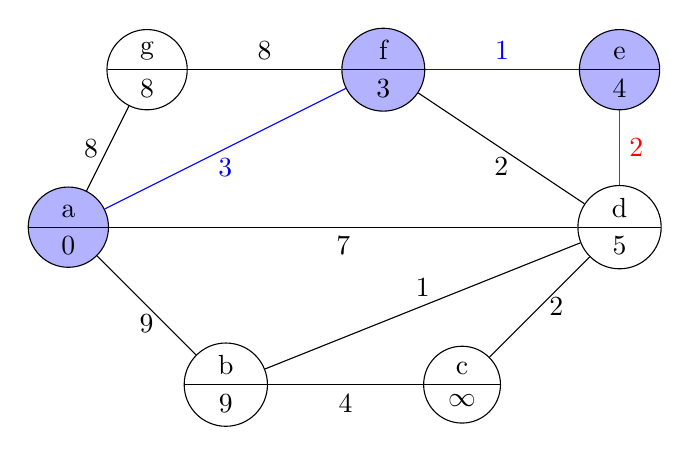
\begin{tikzpicture}
		\draw (0,0) node [state with output, fill=blue!30] (a) {a \nodepart{lower} 0};
		\draw (2,-2) node [state with output] (b) {b \nodepart{lower} 9};
		\draw (5,-2) node [state with output] (c) {c \nodepart{lower} $\infty$};
		\draw (7,0) node [state with output] (d) {d \nodepart{lower} 5};
		\draw (7,2) node [state with output, fill=blue!30] (e) {e \nodepart{lower} 4};
		\draw (4,2) node [state with output, fill=blue!30] (f) {f \nodepart{lower} 3};
		\draw (1,2) node [state with output] (g) {g \nodepart{lower} 8};

		\draw
			(a) edge node [below] {9} (b)
			(a) edge node [left] {8} (g)
			(a) edge [color=blue] node [below] {3} (f)
			(b) edge node [below] {4} (c)
			(c) edge node [right] {2} (d)
			(d) edge [color=red] node [right] {2} (e)
			(d) edge node [below] {2} (f)
			(e) edge [color=blue] node [above] {1} (f)
			(f) edge node [above] {8} (g)
			(a) edge node [below] {7} (d)
			(b) edge node [above] {1} (d)
		;
	\end{tikzpicture}
\end{center}

\textbf{Step 5:}
\begin{center}
	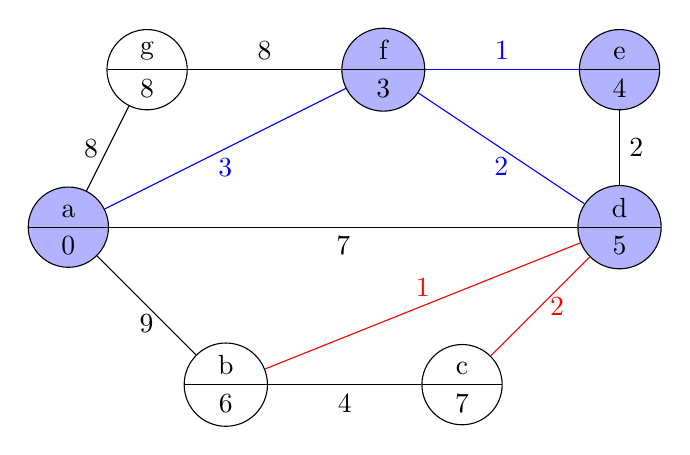
\begin{tikzpicture}
		\draw (0,0) node [state with output, fill=blue!30] (a) {a \nodepart{lower} 0};
		\draw (2,-2) node [state with output] (b) {b \nodepart{lower} 6};
		\draw (5,-2) node [state with output] (c) {c \nodepart{lower} 7};
		\draw (7,0) node [state with output, fill=blue!30] (d) {d \nodepart{lower} 5};
		\draw (7,2) node [state with output, fill=blue!30] (e) {e \nodepart{lower} 4};
		\draw (4,2) node [state with output, fill=blue!30] (f) {f \nodepart{lower} 3};
		\draw (1,2) node [state with output] (g) {g \nodepart{lower} 8};

		\draw
			(a) edge node [below] {9} (b)
			(a) edge node [left] {8} (g)
			(a) edge [color=blue] node [below] {3} (f)
			(b) edge node [below] {4} (c)
			(c) edge [color=red] nnode [right] {2} (d)
			(d) edge node [right] {2} (e)
			(d) edge [color=blue] node [below] {2} (f)
			(e) edge [color=blue] node [above] {1} (f)
			(f) edge node [above] {8} (g)
			(a) edge node [below] {7} (d)
			(b) edge [color=red] node [above] {1} (d)
		;
	\end{tikzpicture}
\end{center}

\textbf{Step 6:}
\begin{center}
	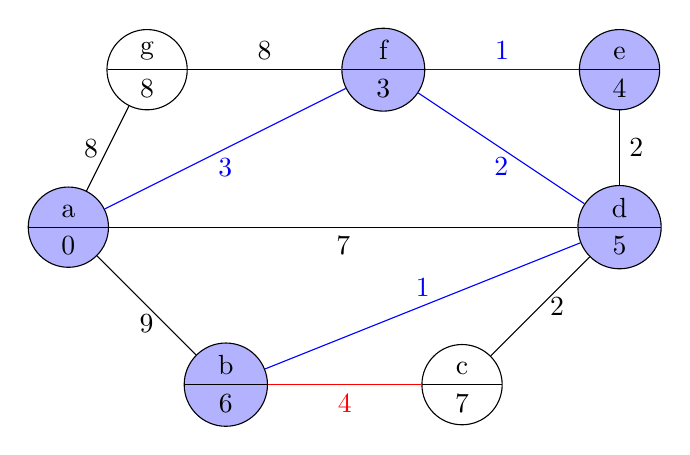
\begin{tikzpicture}
		\draw (0,0) node [state with output, fill=blue!30] (a) {a \nodepart{lower} 0};
		\draw (2,-2) node [state with output, fill=blue!30] (b) {b \nodepart{lower} 6};
		\draw (5,-2) node [state with output] (c) {c \nodepart{lower} 7};
		\draw (7,0) node [state with output, fill=blue!30] (d) {d \nodepart{lower} 5};
		\draw (7,2) node [state with output, fill=blue!30] (e) {e \nodepart{lower} 4};
		\draw (4,2) node [state with output, fill=blue!30] (f) {f \nodepart{lower} 3};
		\draw (1,2) node [state with output] (g) {g \nodepart{lower} 8};

		\draw
			(a) edge node [below] {9} (b)
			(a) edge node [left] {8} (g)
			(a) edge [color=blue] node [below] {3} (f)
			(b) edge [color=red] node [below] {4} (c)
			(c) edge node [right] {2} (d)
			(d) edge node [right] {2} (e)
			(d) edge [color=blue] node [below] {2} (f)
			(e) edge [color=blue] node [above] {1} (f)
			(f) edge node [above] {8} (g)
			(a) edge node [below] {7} (d)
			(b) edge [color=blue] node [above] {1} (d)
		;
	\end{tikzpicture}
\end{center}

\textbf{Step 7:}
\begin{center}
	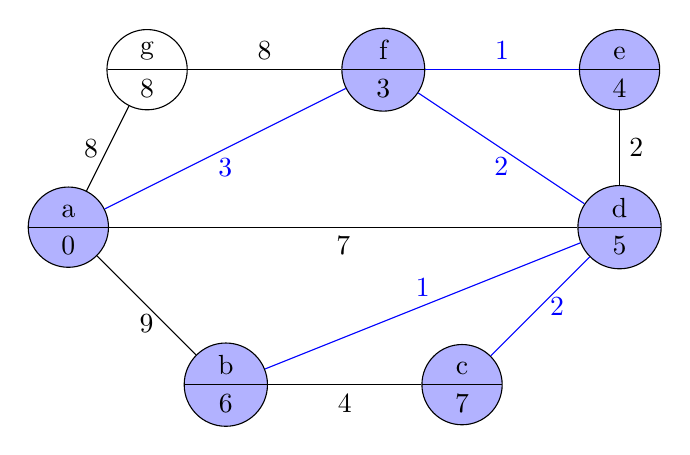
\begin{tikzpicture}
		\draw (0,0) node [state with output, fill=blue!30] (a) {a \nodepart{lower} 0};
		\draw (2,-2) node [state with output, fill=blue!30] (b) {b \nodepart{lower} 6};
		\draw (5,-2) node [state with output, fill=blue!30] (c) {c \nodepart{lower} 7};
		\draw (7,0) node [state with output, fill=blue!30] (d) {d \nodepart{lower} 5};
		\draw (7,2) node [state with output, fill=blue!30] (e) {e \nodepart{lower} 4};
		\draw (4,2) node [state with output, fill=blue!30] (f) {f \nodepart{lower} 3};
		\draw (1,2) node [state with output] (g) {g \nodepart{lower} 8};

		\draw
			(a) edge node [below] {9} (b)
			(a) edge node [left] {8} (g)
			(a) edge [color=blue] node [below] {3} (f)
			(b) edge node [below] {4} (c)
			(c) edge [color=blue] node [right] {2} (d)
			(d) edge node [right] {2} (e)
			(d) edge [color=blue] node [below] {2} (f)
			(e) edge [color=blue] node [above] {1} (f)
			(f) edge node [above] {8} (g)
			(a) edge node [below] {7} (d)
			(b) edge [color=blue] node [above] {1} (d)
		;
	\end{tikzpicture}
\end{center}

\textbf{Step 8:}
\begin{center}
	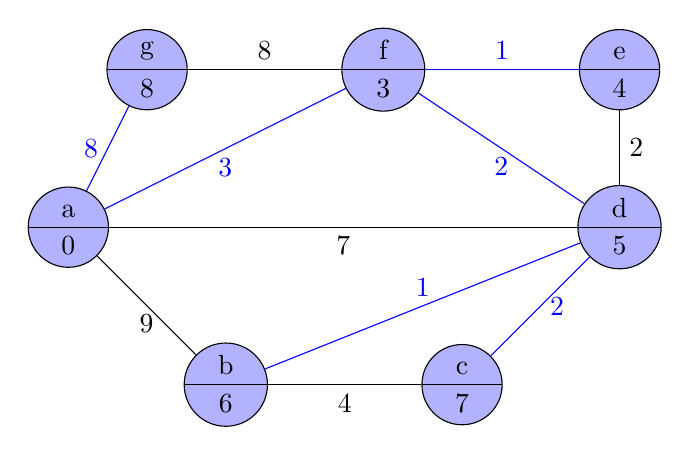
\begin{tikzpicture}
		\draw (0,0) node [state with output, fill=blue!30] (a) {a \nodepart{lower} 0};
		\draw (2,-2) node [state with output, fill=blue!30] (b) {b \nodepart{lower} 6};
		\draw (5,-2) node [state with output, fill=blue!30] (c) {c \nodepart{lower} 7};
		\draw (7,0) node [state with output, fill=blue!30] (d) {d \nodepart{lower} 5};
		\draw (7,2) node [state with output, fill=blue!30] (e) {e \nodepart{lower} 4};
		\draw (4,2) node [state with output, fill=blue!30] (f) {f \nodepart{lower} 3};
		\draw (1,2) node [state with output, fill=blue!30] (g) {g \nodepart{lower} 8};

		\draw
			(a) edge node [below] {9} (b)
			(a) edge [color=blue] node [left] {8} (g)
			(a) edge [color=blue] node [below] {3} (f)
			(b) edge node [below] {4} (c)
			(c) edge [color=blue] node [right] {2} (d)
			(d) edge node [right] {2} (e)
			(d) edge [color=blue] node [below] {2} (f)
			(e) edge [color=blue] node [above] {1} (f)
			(f) edge node [above] {8} (g)
			(a) edge node [below] {7} (d)
			(b) edge [color=blue] node [above] {1} (d)
		;
	\end{tikzpicture}
\end{center}

\section*{Question 15.3}

Here is an example where the claim can be false.

\begin{center}
	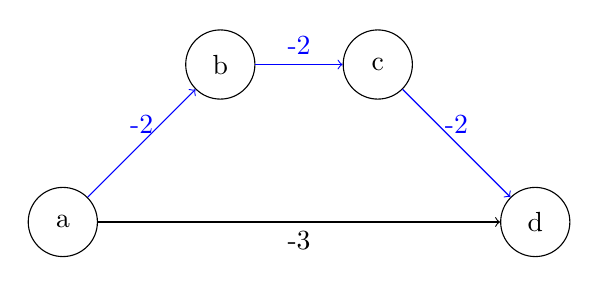
\begin{tikzpicture}[auto]
		\draw (0,0) node [state] (a) {a};
		\draw (2,2) node [state] (b) {b};
		\draw (4,2) node [state] (c) {c};
		\draw (6,0) node [state] (d) {d};

		\draw[->]
			(a) edge [color=blue] node [above] {-2} (b)
			(b) edge [color=blue] node [above] {-2} (c)
			(c) edge [color=blue] node [above] {-2} (d)
			(a) edge node [below] {-3} (d)
		;
	\end{tikzpicture}
\end{center}

This is a directed acyclic graph. 
The shortest path from $a$ to $d$ is $a \rightarrow b \rightarrow c \rightarrow d$ with weight -6.
The lower path, $a \rightarrow d$, has weight -3.

However, if we add a constant weight to all edges to make them positive, the graph becomes:
\begin{center}
	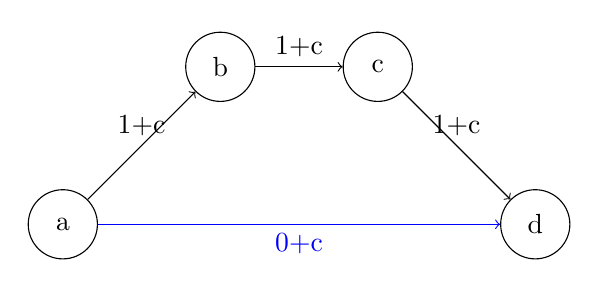
\begin{tikzpicture}[auto]
		\draw (0,0) node [state] (a) {a};
		\draw (2,2) node [state] (b) {b};
		\draw (4,2) node [state] (c) {c};
		\draw (6,0) node [state] (d) {d};

		\draw[->]
			(a) edge node [above] {1+c} (b)
			(b) edge node [above] {1+c} (c)
			(c) edge node [above] {1+c} (d)
			(a) edge [color=blue] node [below] {0+c} (d)
		;
	\end{tikzpicture}
\end{center}

Here $c$ represents a non-negative constant.
In this case, the shortest path from $a$ to $d$ is $a \rightarrow d$ with weight $c$.
The upper path, $a \rightarrow b \rightarrow c \rightarrow d$, has weight $3 + 3c$.

The real problem with this claim is that:
for two distinct paths $p_1$ and $p_2$ from $s$ to $t$, the number of edges in $p_1$ and $p_2$ can be different.
Let $n_1$ and $n_2$ be the number of edges in $p_1$ and $p_2$ respectively.
If the sum of weights of edges in $p_1$ is $W_1$ before adding a constant weight $c$ to all edges,
then the sum of weights of edges in $p_1$ after adding $c$ is $W_1 + n_1c$.
Similarly, the sum of weights of edges in $p_2$ after adding $c$ is $W_2 + n_2c$.
In this case, the difference $W_1 - W_2$ will change after adding $c$, becomes $W_1 + n_1c - W_2 - n_2c = (W_1 - W_2) + (n_1 - n_2)c$.
It is possible that $W_1 - W_2 < 0$ but $n_1 - n_2 > 0$, making $W_1 + n_1c - W_2 - n_2c > 0$.
Then the shortest path changes from $p_1$ to $p_2$ after adding $c$.
\end{document}